\documentclass[final]{siamltex}
%\documentclass[12pt]{article}
\usepackage[dvips]{attachfile2}
\usepackage{mathdef}

\let\orightarrow\rightarrow
\let\omapsto\mapsto
\usepackage{breqn}
\let\rightarrow\orightarrow
\def\longrightarrow{\relbar\joinrel\joinrel\joinrel\orightarrow}
\let\mapsto\omapsto
\usepackage{hyperbreqn}

\def\be{\begin{dmath*}}
\def\ee{\end{dmath*}}
\def\bel{\begin{dmath}}
\def\eel{\end{dmath}}
\def\bec{\begin{dmath*}[compact]}
\let\eec\ee
\def\belc{\begin{equation}}
\def\eelc{\end{equation}}

\def\bg{\begin{dgroup*}}
\def\eg{\end{dgroup*}}
\def\bgl{\begin{dgroup}}
\def\egl{\end{dgroup}}
\def\bs{\begin{dsuspend}}
\def\es{\end{dsuspend}}
\def\no{\hiderel}

\newcommand{\Fourier}[0]{\mathcal{F}}

\begin{document}

%\title{Implicit Dealiasing of Fourier-Based Convolutions}
\title{Efficient Dealiased Convolutions without the Padding}
\author{John C. Bowman and Malcolm Roberts}
\maketitle

\begin{abstract}
An algorithm is described for dealiasing linear convolution sums
without the expense of conventional zero-padding or phase-shift
techniques. For one-dimensional in-place convolutions, the memory
requirements are identical with the zero-padding technique, with the important
distinction that the additional work memory need not be contiguous with the
data. This decoupling of the data and work arrays significantly reduces
the memory and computation time required to evaluate higher-dimensional
in-place convolutions. The technique also allows one to efficiently dealias the
hyperconvolutions that arise on Fourier transforming arbitrary powers.
Implicitly padded convolutions can be built on top of state-of-the-art
fast Fourier transform libraries: vectorized multidimensional implementations
for the complex and centered Hermitian (pseudospectral) cases have
been implemented in the open-source software {\tt fftw++}.
\end{abstract} 

\begin{keywords} 
dealiasing, zero padding, convolution, hyperconvolution, fast Fourier transform,
pseudospectral method, in-place transform, bit reversal
\end{keywords}

\begin{AMS}
65R99,65T50
%15A15, 15A09, 15A23
\end{AMS}

\pagestyle{myheadings}

% Add ref to Cooley--Tukey
% We should also implement a unshifted Hermitian convolution.

%use out-of-place Fourier transforms where possible (percent?)

% decoupling is more convenient for the user, 
% 

%padding to smooth data vs. chirp-z algorithm

%
%highly optimized

%avoids inconvenience of and extra copying required by zero padding

% CRAY power-of-2 stride issue
% Supports efficient convolutions of power of 2 sizes
%
% memory requirements of phase-shift \cite{Patterson and Orszag 71} (doubles
% memory usage).

% Think about parallelization issues (another advantage of removing zeros).

\section{Introduction}
Discrete linear convolution sums based on the fast Fourier transform (FFT)
algorithm have become important tools for image filtering, digital signal
processing, and correlation analysis. They are also widely used in
computational physics to solve nonlinear partial differential equations
such as the Navier--Stokes equations in periodic domains. In some of these
applications, notably direct numerical pseudospectral simulations of fluid
turbulence, memory usage is a critical limiting factor: in-place
multidimensional Fourier transforms are typically used to reduce the memory
footprint of the required spectral convolutions.

Because the discrete convolution, which produces cyclic output from cyclic
input, is applied to nonperiodic (wavenumber-space) data, it is important
to remove aliases from the convolution. Typically the data array is
extended by padding it with enough zeros so that the wave beats of the
the positive frequencies cannot wrap around and contaminate
the negative frequencies. The convolution is then performed using a
correspondingly larger Fourier transform size. Alternatively, phase
shift dealiasing \cite{Patterson71,Canuto} can be used to cancel out the
aliasing errors between two convolutions with two different phase
shifts. However, this second technique is rarely used in practice, since in
addition to doubling the memory requirements, it is computationally more
expensive ($15N\log_2 N$ operations) than zero padding
($\fr{45/4}N\log_2 N$ operations) \cite[p.~136]{Canuto}. 

An explicit application of the zero-padding technique has the rather
obvious inefficiency of summing over a large number of data values that
are known {\it a priori\/} to be zero.
To a frequently asked question by FFT users who want to avoid this
unnecessary expense in computing a dealiased convolution,
Steven G. Johnson has provided this
answer\cite{http://www.fftw.org/pruned.html}:
\begin{quotation}
{\it
The most common case where people seem to want a pruned FFT is for
zero-padded convolutions, where roughly 50\% of your inputs are zero (to
get a linear convolution from an FFT-based cyclic convolution). Here, a
pruned FFT is hardly worth thinking about, at least in one dimension. In
higher dimensions, matters change (e.g. for a 3d zero-padded array about
1/8 of your inputs are non-zero, and one can fairly easily save a factor of
two or so simply by skipping 1d sub-transforms that are zero).
}
\end{quotation}

The reasoning behind the assertion that such one-dimensional pruned FFTs
are not worth thinking about is that if $K$ of the $N$ inputs are zero,
the computational cost is reduced only from $N\log N$ to $N\log K$.
For example, if $K=N/2$, the savings is a minuscule $1/\log_2 N$.
Nevertheless, in this work we demonstrate that pruning the zero-padded
elements of one-dimensional convolutions is indeed worth thinking about,
primarily because it provides a more effective building block for constructing
multidimensional convolutions.

The key observation is that, although the memory usage of our implicitly
padded 1D convolution is identical to that for a conventional explicitly
padded convolution, the additional temporary memory need not be contiguous
with the user data.  In a multidimensional context, this external work
buffer can be reused for other one-dimensional convolutions.
As a result, for dimensions greater than one, the memory usage of our
unshifted (centered) convolution is asymptotically one-half (two-thirds)
of the memory requirements imposed by zero padding.
Of course, if memory savings alone were the goal, this savings could
also be achieved with explicit zero padding by copying the data for the
innermost convolution to an external padded buffer, but such extra data
communication turns out to be prohibitively expensive. The fact that our
one-dimensional convolution does not require this extra copying is the key
feature that was exploited to obtain simultaneous improvements in memory
usage and performance.

Nevertheless, the task of writing an efficient implicitly padded one-dimensional
convolution is onerous, particularly if one tries to compete with an
explicitly problem-dependent and architecture-adaptive FFTW algorithm such
as the award-winning \cite{FFTW} library, which empirically predetermines a
near optimal butterfly graph at each subdivision. Effectively one wants to
perform the first FFT subdivision manually, dropping the zero terms and
leaving the inner transforms to be computed with the usual library
routine. But this places an artificial restriction, at least at the highest
subdivision, on the possible adaptive algorithm that can be
used. Fortunately, there are a number of features of our algorithm that
help to offset this disadvantage. First, since the goal is to produce a
convolution, bit-reversal for the manual (highest) subdivision is
unnecessary: the scrambled Fourier subtransforms of the two input vectors
can be multiplied together as they are produced (perhaps while are still
accessible in the cache). Second, the implicit method allows most (four out
of six for the complex unshifted case and seven out of nine for the
Hermitian centered case) of the subtransforms for an in-place convolution
to be computed as out-of-place transforms, which are typically faster than
in-place transforms.  These savings helped keep our one-dimensional in-place
implicit convolution competitive with the explicitly padded convolution
based on the same highly optimized library.

\section{1D Implicitly Padded Convolution}
\subsection{Complex convolution}

In the unshifted case, the Fourier origin is at the first index and the input
data vectors of length $m$ must each be zero-padded to length $N\ge 2m-1$ to
prevent the wavenumber $m-1$ from beating with itself to
affect mode~$N=0\mod n$. However, since power-of-two FFT transforms in practice
yield the most efficient implementations, it is typically
better to extend the padding to $N=2m$.

In terms of the $N$th primitive root of unity,
$\zeta_N\doteq \exp\(2 \pi i/N\)$, we define the
unnormalized discrete inverse Fourier transform
$$
u_j\doteq\sum_{k=0}^{N-1}\zeta_N^{jk} \hat u_k\qquad j=0,\ldots,N-1.
$$
($\doteq$ indicates a definition).
Our method exploits the properties that $\zeta_N^r=\zeta_{N/r}$ and
$\zeta_N^N=1$.

If $\hat u_k=0$ for $k \ge m$ then we can discard these zero modes by
decimating in frequency:
\belc
u_{2\ell}
=\ds\sum_{k=0}^{m-1}\zeta_m^{\ell k} \hat u_k,
\qquad
u_{2\ell+1}
=\ds\sum_{k=0}^{m-1}\zeta_m^{\ell k} \zeta_N^k\hat u_k
\qquad
(\ell=0,1,\ldots m-1).\label{cconv1inv}
\eelc
Since this requires computing two subtransforms, each of size $m$,
the overall computational scaling is of order $2m\log m=N\log(m)$.

The odd and even terms of the convolution can then be computed separately
(without the need for a bit reversal stage), multiplied term-by-term, and
transformed back to Fourier space using the forward transform
\bel
N\hat u_k=\sum_{j=0}^{N-1}\zeta_N^{-kj} u_j
=\sum_{\ell=0}^{m-1}\zeta_N^{-2k\ell} u_{2\ell}
+\zeta_N^{-k}\sum_{\ell=0}^{m-1}\zeta_N^{-2k\ell} u_{2\ell+1}
=\sum_{\ell=0}^{m-1}\zeta_m^{-k\ell} u_{2\ell}
+\zeta_N^{-k}\sum_{\ell=0}^{m-1}\zeta_m^{-k\ell} u_{2\ell+1}
\qquad k\no=0,\ldots,\fr{N}{2}-1.\label{cconv1}
\eel
One can thus compute a dealiased convolution of (unpadded) length $m$ using
for each input vector two blocks of size $m$ instead of one block of size $2m$.
This seemingly trivial distinction is the key to the improved efficiency
and reduced storage requirements of the higher-dimensional implicit
convolutions describe in Sections~\ref{conv2} and~\ref{conv3}.

Referring to the computation times shown in Figure~\ref{timing1c},
we see that the implicit padding algorithm, \Eqs{cconv1} and~\ref{cconv1inv},
is quite competitive with convolution by explicit padding. Both the FFTW library
and the convolution layer we built on top of it were compiled with the
Intel C/C++ Compiler and optimization options and run on a 64-bit Intel
processor. Like the FFTW library, our algorithm was vectorized with specialized
single-instruction multiple-data (SIMD) code.

\begin{figure}[htbp]
  \begin{center}
    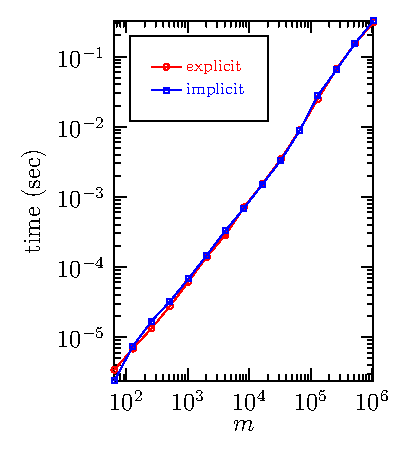
\includegraphics{timing1c}
    \caption{Comparison of computation times for explicitly and implicitly
dealiased complex in-place 1D convolutions of two vectors of
(unpadded) length $m$.}
    \label{timing1c}
  \end{center}
\end{figure}

\subsection{Centered Hermitian convolution}

In this frequently encountered case (relevant to the pseudospectral
method), the input data length is odd, say $2m-1$, with the Fourier origin
at index $m-1$. One then needs to pad to $N\ge 3m-2$ to prevent the
wavenumber $m-1$ from beating with itself to affect the most negative
(first) wavenumber, $-m+1$. Since the ratio of the number of physical to
total modes, $(2m-1)/(3m-2)$ is asymptotic to $2/3$ for large $m$, the
explicit padding technique is often referred to as the {\it $2/3$ padding
rule}.  This padding ratio turns out to work particularly well with the
Hermiticity condition, $\hat{u}_{-k}=\overline{\hat{u}_k}$, which guarantees
that the $x$-space data is real-valued.
% Consider a wavenumber-truncated
%vector ranging from $k=-(m-1)$ to $k=m-1$, which 
%has $2m-1$ elements.

For explicit padding, one typically choses the padded vector length
$N$ to be a power of $2$, with $m=\floor{(n+2)/3}$. However, for implicit
padding, it is advantageous to choose $m$ itself to be a power of $2$
since the algorithm reduces to computing $m$-length FFTs.
Moreover, it is convenient to pad implicitly beyond $3m-2$ to $N=3m$
as this allow the use of a radix $3$ subdivision at the highest level, so
that only two of the three subtransforms of length $m$ need to be retained. 

Given that $\hat u_k=0$ for $k\ge m$, the backwards (complex-to-real) transform
may be expressed using the substitution $k'=m+k$ as 
\bec
u_{3\ell +r}\no=\sum_{k=-m+1}^{m-1}\z_m^{\ell k} \z_N^{rk} \hat u_k
=\sum_{k'=1}^{m-1}\z_m^{\ell k'} \z_N^{r(k'-m)} \hat u_{k'-m}
+\sum_{k=0}^{m-1}\z_m^{\ell k} \z_N^{rk} \hat u_k
=\sum_{k=1}^{m-1}\z_m^{\ell k} \z_N^{-r(m-k)} \hat u_{m-k}^*
+\sum_{k=0}^{m-1}\z_m^{\ell k} \z_N^{rk} \hat u_k
=\sum_{k=0}^{m-1}\z_m^{\ell k} \(w_{k,r}+w_{m-k,r}^*\),
\ee
where
$$
w_{k,r}=\z_N^{rk} \(\hat u_k-\half \hat u_0\d_{k,0}\).
$$
The forwards transform becomes
\be
N\hat u_k=\sum_{j=0}^{N-1}\zeta_N^{-kj} u_j
=\sum_{r=-1}^{1}\zeta_N^{-rk}\sum_{\ell=0}^{m-1}\zeta_N^{-3\ell k} u_{3\ell+r}
=\sum_{r=-1}^{1}\zeta_N^{-rk}\sum_{\ell=0}^{m-1}\zeta_m^{-\ell k} u_{3\ell+r}
\qquad k\no =0,\ldots,m-1.
\ee




$$
u_j=\sum_{k=0}^{N-1}\zeta_N^{jk} \hat u_k
=\sum_{k=0}^{2m-1}\zeta_N^{jk} \hat u_k
$$
Then 
\bel
u_{3\ell}= \sum_{k=0}^{2m-1}\z_{3m}^{3\ell k} \hat u_k
=\sum_{k=0}^{m-1}\z_m^{\ell k} \hat u_k
+\sum_{k=m}^{2m-1}\z_m^{\ell k} \hat u_k
=\sum_{k=0}^{m-1}\z_m^{\ell k} \hat u_k
+\sum_{k=0}^{m-1}\z_m^{\ell (k+m)} \hat u_{k+m}
=\sum_{k=0}^{m-1}\z_m^{\ell k} \(\hat u_k+\hat u_{k+m}\).\label{DFTm}
\eel
Equation~\ref{DFTm} is a DFT of length $m$,
each requiring $m\log m$ operations. Following a similar procedure,
with $r=1$ or $r=2$,
\bel
\label{dfft23g}
u_{3\ell +r}\no=
 \sum_{k=0}^{m-1}\z_m^{\ell k} \(\z_N^{rk} \hat u_k + \z_N^{r(k+m)}\hat u_{k+m}\)
\eel
Thus, the total number of operations is $3 m \log m = N \log\frac{N}{3}$.

The forward Fourier transform appears as
\be
N\hat u_k=\sum_{j=0}^{N-1}\zeta_N^{-kj} u_j
=\sum_{r=0}^{2}\zeta_N^{-rk}\sum_{\ell=0}^{m-1}\zeta_N^{-3\ell k} u_{3\ell+r}
=\sum_{r=0}^{2}\zeta_N^{-rk}\sum_{\ell=0}^{m-1}\zeta_m^{-\ell k} u_{3\ell+r}
\qquad k\no =0,\ldots,pm-1.
\ee

The computation times for implicit padding of a centered is compared with
explicit zero padding in Figure~\ref{timing1r}. For the intended
application to partial differential equations, there is flexibility in the
choice of the exact convolution size. This is why we consider for each
algorithm only those vector lengths that maximize performance.

\begin{figure}[htbp]
  \begin{center}
    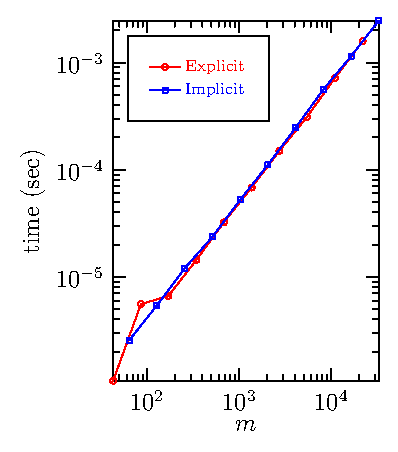
\includegraphics{timing1r}
    \caption{Comparison of computation times for explicitly and implicitly
dealiased centered Hermitian in-place 1D convolutions of two vectors of
(unpadded) length $2m-1$.}
    \label{timing1r}
  \end{center}
\end{figure}

On the other hand, for those applications where the size of the convolution
is dictated by external criteria, implicit padding effectively expands the
set of efficient convolutions sizes to include integral powers of $2$, a
case of practical significance. The existence of implicit convolutions in
fact nullifies the argument of Canuto...
% Address slightly misleading implication of Canuto page 136
% (dealiased.pdf: p.20) regarding power of 2 transforms (depends on
% application).

\newpage
\subsubsection{1D Complex to Real Transforms of 2/3 Dealiased Data}


Note: without the hermiticity condition, the backwards transform is
\bec
u_{3\ell +r}\no=\sum_{k=-m+1}^{m-1}\z_m^{\ell k} \z_N^{rk} \hat u_k
=\sum_{k'=1}^{m-1}\z_m^{\ell k'} \z_N^{r(k'-m)} \hat u_{k'-m}
+\sum_{k=0}^{m-1}\z_m^{\ell k} \z_N^{rk} \hat u_k
=\sum_{k=0}^{m-1}\z_m^{\ell k} w_{k,r},
\ee
where
$$
w_{k,r}=
\cases{
\hat u_0&if $k=0$,\cr
\z_N^{rk}(\hat u_k+\z_3^{-r}\hat u_{k-m})&if $1\le k\le m-1$.\cr
}
$$
and the forwards transform is
\be
N\hat u_k=\sum_{j=0}^{N-1}\zeta_N^{-kj} u_j
=\sum_{r=-1}^{1}\zeta_N^{-rk}\sum_{\ell=0}^{m-1}\zeta_m^{-\ell k} u_{3\ell+r}
\qquad k\no =-m+1,\ldots,m-1.
\ee



\subsubsection{2D Complex to Real Transforms of 2/3 Dealiased Data}
The Hermiticity condition is now $\hat{u}_{-k,-\ell}=\hat{u}^*_{k,\ell}$.
The procedure is analagous as in 1D,
where we interpret each index as a vector, add dot products,
split the two-dimensional sum into lower and upper halves, and use the
change of variables $\vk=(m_x,m_y)+\vk'$.
\begin{comment}
\bec
u_{3u+r,3v+s}\no=\sum_{k=-m-1}^{m-1}\sum_{\ell=-m-1}^{m-1}
\z_m^{u k} \z_m^{v \ell} \z_N^{rk} \z_N^{s\ell} \hat u_{k,\ell}
=\sum_{k=-m-1}^{m-1}\z_m^{u k}\z_N^{rk}  
\sum_{\ell=1}^{m-1} \z_m^{v \ell} \z_N^{s(\ell'-m)} \hat u_{k,\ell'-m}
+\sum_{k=-m-1}^{m-1}\z_m^{u k}\z_N^{rk}
\sum_{\ell=0}^{m-1} \z_m^{v \ell} \z_N^{s\ell} \hat u_{k,\ell}
=\sum_{k=-m-1}^{m-1}\z_m^{-u k}\z_N^{-rk}  
\sum_{\ell=1}^{m-1} \z_m^{v \ell} \z_N^{-s(m-\ell')} \hat u_{k,m-\ell'}^*
+\sum_{k=-m-1}^{m-1}\z_m^{u k}\z_N^{rk}
\sum_{\ell=0}^{m-1} \z_m^{v \ell} \z_N^{s\ell} \hat u_{k,\ell}
\ee
\end{comment}

%Our 1024x1024 complex convolution is now 48\% faster (the pruned one is
%27\% faster)!

\begin{figure}[htbp]
  \begin{center}
    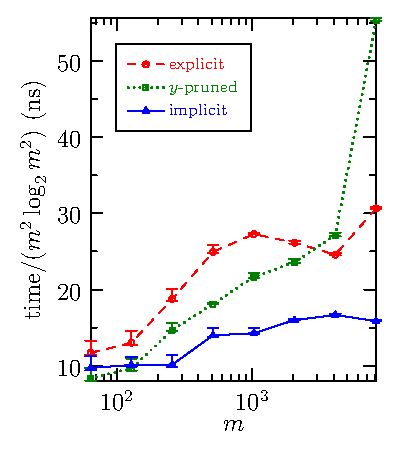
\includegraphics{timing2c}
    \caption{Comparison of computation times for explicitly and implicitly
dealiased complex in-place 2D convolutions of two vectors of
(unpadded) length $m\times m$.}
    \label{timing2c}
  \end{center}
\end{figure}

\begin{figure}[htbp]
  \begin{center}
    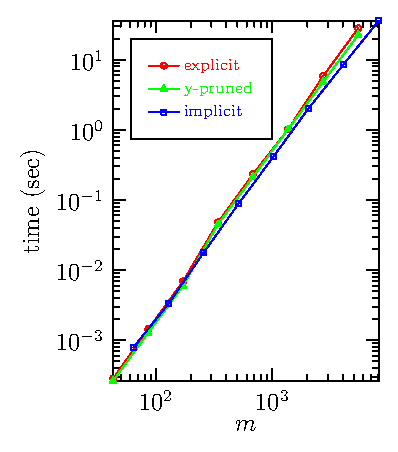
\includegraphics{timing2r}
    \caption{Comparison of computation times for explicitly and implicitly
dealiased centered Hermitian in-place 2D convolutions of two vectors of
(unpadded) length $(2m-1)\times (2m-1)$.}
    \label{timing2r}
  \end{center}
\end{figure}


\newpage
\subsection{$p/q$ Dealiased Data}

In general, consider a ``$p/q$'' padding in which $N=qm$, and only $pm$ modes
are non-zero, with $p$ and $q$ relatively prime. Consider $u_{q\ell+r}$, with
$\ell=0 \dots m-1$, $r=0 \dots q-1$.
Then
\be
u_{q\ell+r} = \sum_{k=0}^{N-1}\z_N^{(q\ell+r)k} \hat u_k
= \sum_{k=0}^{pm-1}\z_{qm}^{(q\ell+r)k} \hat u_k
= \sum_{k=0}^{pm-1}\z_m^{\ell k}\z_{N}^{rk} \hat u_k
= \sum_{\a=0}^{p-1} \sum_{k=\a m}^{(\a+1)m-1}\z_m^{\ell k}\z_{N}^{rk} \hat u_k
= \sum_{\a=0}^{p-1} \sum_{\k=0}^{m-1}\z_m^{\ell (\k+\a m)}\z_{N}^{r(\k+\a m)}
\hat u_{\k+\a m}
%=  \sum_{\a=0}^{p-1}\z_N^{r \a m} \sum_{\k=0}^{m-1}\z_m^{\ell\k}\z_N^{r\k}\hat u_{\k+\a m}
=  \sum_{\k=0}^{m-1}\z_m^{\ell\k}\sum_{\a=0}^{p-1}\z_N^{r(\k+\a m)} \hat u_{\k+\a m}
\ee .
Note that, in the last line, we have the choice of which $\z$ to use, since
$\z_q^{r \a}=\z_N^{r \a m}$. Since there are $m$ choices of $r$ and $q$ choices
for $\ell$, we are left with $mq=N$ FFTs of length $p$, leaving on the order
of $N \log p = N \log (N/q)$ operations.  Again, while the computational
savings is only marginal, this formulation affords signficant improvements
in memory use and parallelizability.

The forward Fourier transform appears as
\be
N\hat u_k=\sum_{j=0}^{N-1}\zeta_N^{-kj} u_j
=\sum_{r=0}^{q-1}\zeta_N^{-rk}\sum_{\ell=0}^{m-1}\zeta_N^{-q\ell k} u_{q\ell+r}
=\sum_{r=0}^{q-1}\zeta_N^{-rk}\sum_{\ell=0}^{m-1}\zeta_m^{-\ell k} u_{q\ell+r}
\qquad k\no =0,\ldots,pm-1.
\ee

%TODO: I think that this can be generalized in the following fashion:
%if $m$ of the $N$ modes are non-zero, let $p=N/\gcd(m,N)$. Then we
%have can divide up the DFT into $p$ DFTs of length $m$. Must work out
%the details.




\section{2D, 2/3-dealiased transforms}
Our goal is to apply this to dealiased pseudospectral simulations. If we 
avoid moving the $k$-space origin to the middle of the array, the Fourier
data is sparse, with a square of length $2/3$ being non-zero. Suppose that 
the first FFT is done in the $x$ direction.  Then, $1/3$ of the transforms
are zero, and can be ignored. The remaining transforms are $2/3$ dealiased,
each of which can be done with $n \log (2 n/3)$ operations. This leaves
the upper $1/3$ modes set to zero.  The final transform, done in the 
$y$-direction, takes $n \log(2 n/3)$ operations.  See figure \ref{dealias2d}.
The total cost is then
\be
\frac{2 n}{3} \log \frac{2 n}{3} +  n \log \frac{2 n}{3}
=\frac{5n}{3} \log \frac{2 n}{3},
\ee
using the dealiased FFT, as opposed to $2 n \log n$ for the naive FFT. This 
is $1/6$ faster, while using significantly less memory. Moreover, the
intermediary, $1/3$-sparse buffer can be kept allocated as an intermediary
buffer for all necessary transformations.
\begin{figure}[htbp]
  \begin{center}
    \includegraphics{dealias2d}
    \caption{Procedure for transforming 2D dealiased arrays.}
    \label{dealias2d}
  \end{center}
\end{figure}

\section{Conclusions}
In this work we develop an efficient method for avoiding explicit zero
padding in multidimensional convolutions, saving both memory and
computation time.

\end{document}

%Self-sorting in-place fast fourier transforms
%Source 	SIAM Journal on Scientific and Statistical Computing archive
%Volume 12 ,  Issue 4  (July 1991) table of contents
%Pages: 808 - 823  
%Year of Publication: 1991
%ISSN:0196-5204 

% LocalWords:  dealiasing dealias hyperconvolutions Hermitian fftw FFT priori
% LocalWords:  hyperconvolution nonperiodic FFTs noncentered subtransforms
% LocalWords:  unpadded
